% write your paper in here

\chapter{Scaffolding assemblies with Hi-C}

Recent genome assembly projects generally aim to achieve chromosome-level scaffolds, and Hi-C scaffolding is a major step to reach this goal. This method has been included successfully in many studies for bacteria, yeasts, plants, animals, and is part of assembly pipelines for several consortia, such as the Vertebrate Genome Project \cite{vgp} and the Darwin Tree of Life \cite{dtol}. instaGRAAL is an improved version of GRAAL \cite{graal}, a Hi-C scaffolder based on MCMC. GRAAL iteratively tests arrangements of the fragments until converging to an assembly with a higher likelihood based on contact frequencies. Two main aspects have been ameliorated: first, instaGRAAL is more computationally efficient, enabling it to handle larger genomes (over 1 Gb); second, it introduces a module to automatically refine the scaffolds based on the input contigs and reduce misassemblies. In the following paper, instaGRAAL was tested on assemblies of the brown algae \textit{Desmarestia herbacea} and \textit{Ectocarpus} sp., and was benchmarked along SALSA2 \cite{salsa2} on a human; it systematically yielded chromosome-level scaffolds. \\
I contributed to testing instaGRAAL, in particular on a human genome, and I also improved the documentation to make it more accessible for new users.

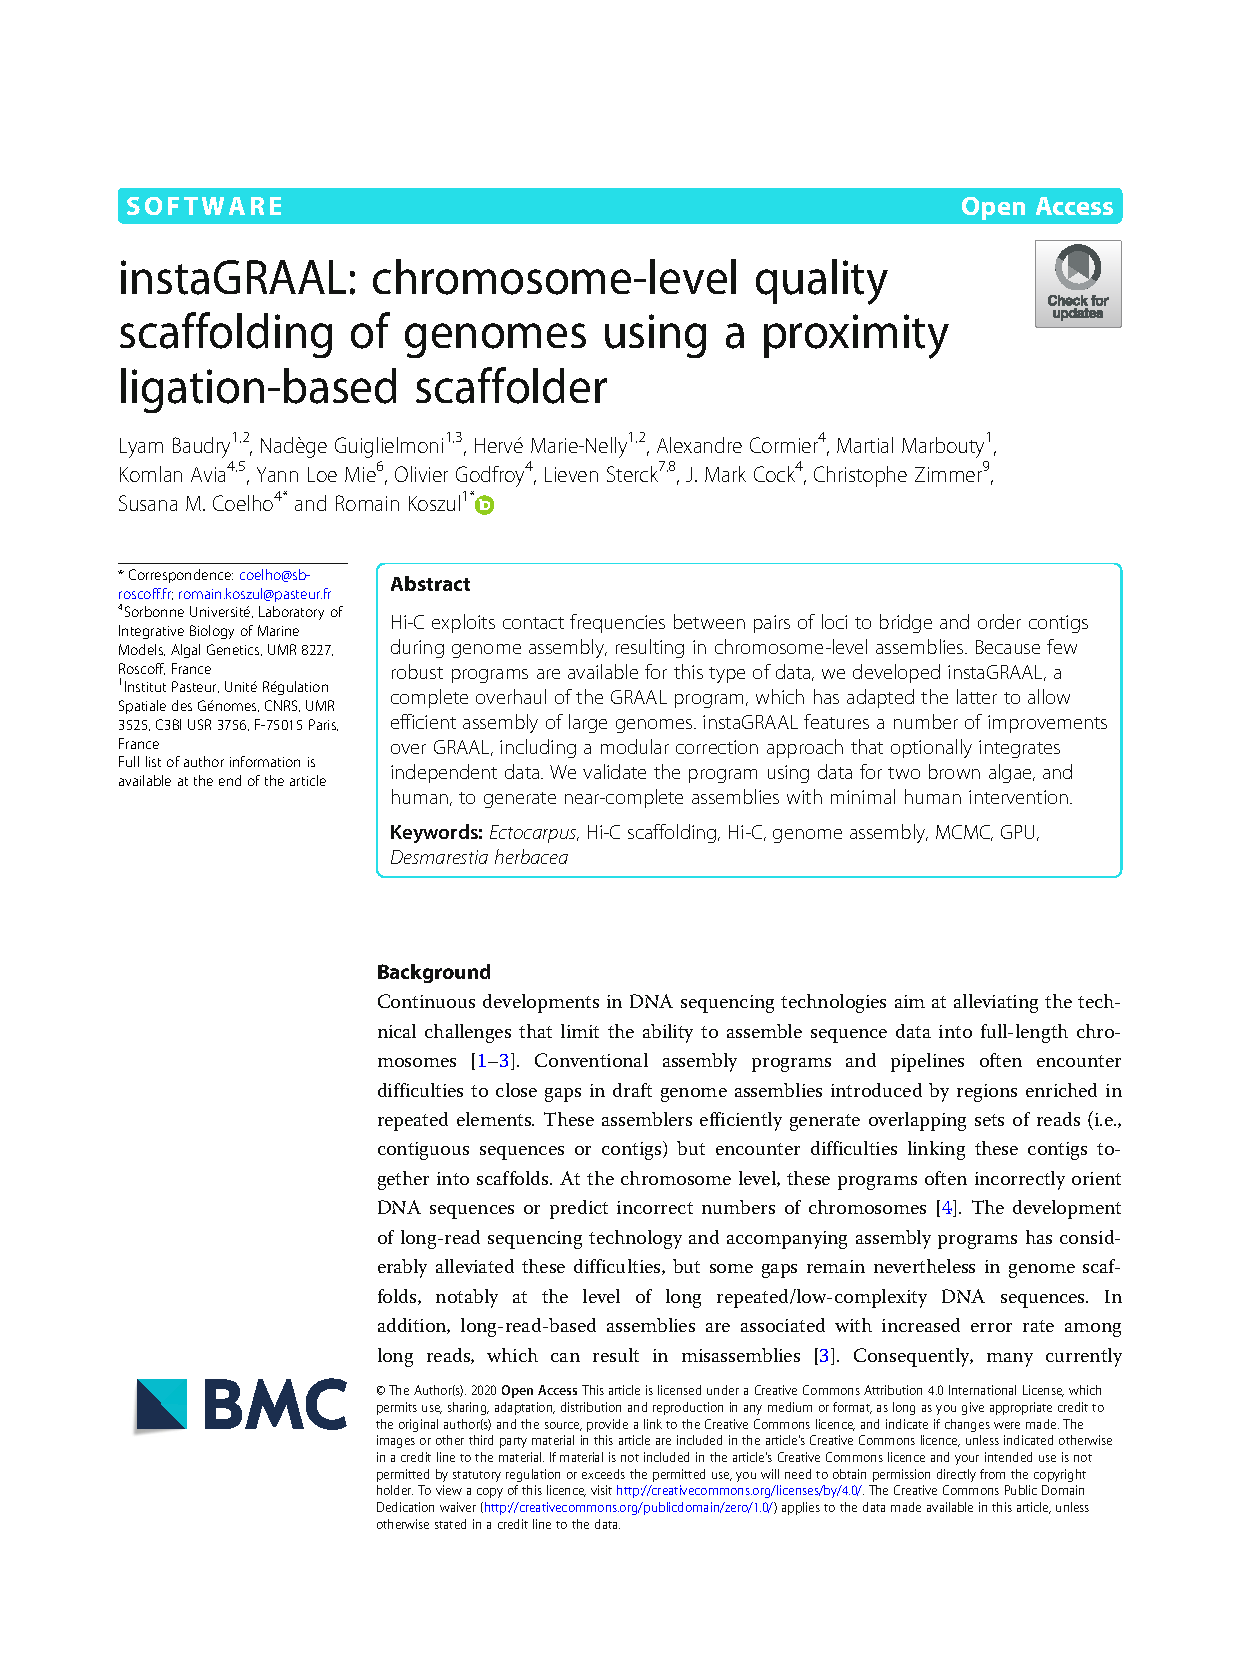
\includepdf[pages=-, pagecommand={}]{articles/instagraal.pdf}